\section{Experimental Methodology}
\label{sec:method}

In this section we discuss our methodological decisions.

Our methodology answers the following questions:
\begin{itemize}
	\item{What workloads did we choose to run for our experiments and why?}
	\item{How do we investigate the memory per core problem?}
	\item{How do we choose the configurations for running the co-located experiments?}
	\item{How do we decide what percentage of total cgroup DRAM to use for Java Heap for each cgroup?}
%	\item{What kind of metrics did we use to analyze performance and why?}
	\item{Is cost a contributing factor to pursuing higher throughput for a server?}
\end{itemize}

\subsection{Workloads}
For our experiments with Spark, we selected four specific workloads from two
different categories of the Spark Bench suite \cite{Spark-Bench}: Page Rank (PR) and Connected
Component (CC) from GraphX \cite{GraphX} and Linear Regression (LinR) and Logistic Regression (LogR)
from MLLib \cite{MLLib}. For Giraph we choose PageRank and Community detection 
using label propagation (CDLP) from LDBC Graphalytics \cite{ldbc}. The primary reason for selecting these workloads for Spark is that
they represent different types of algorithms: PR and CC are graph-based workloads, while LinR and LogR are machine learning
workloads. Giraph is a graph processing framework so we only used graph workloads. All of these
workloads are well-established and commonly used for benchmarking big
data analytics systems, making them a suitable choice for our
experiments. Overall, the selection of these workloads allows us to
evaluate the performance of Spark and Giraph in a variety of contexts. Furthermore it allows us to
provide insights into the performance of both frameworks with or without using TeraHeap.


\subsubsection{PageRank}
PageRank is a widely used graph-based algorithm that measures the
importance of nodes in a network. It has become a popular benchmark
for evaluating the performance of distributed systems, including big
data analytics systems like Apache Spark and Giraph. PageRank is computationally
intensive and requires significant memory and I/O resources, making it
a suitable workload for evaluating performance of managed big data frameworks. Additionally, PageRank is a
common algorithm in real-world applications, such as search engines
and social networks, making it relevant for practical use cases.

\subsubsection{LinearRegression}
LinearRegression is a machine learning algorithm that is used to
predict numerical values based on input data. It is a well-known and
widely used algorithm in machine learning, and is commonly used for
regression analysis in fields such as economics, finance, and
engineering. LinearRegression is computationally intensive and
requires significant memory and I/O resources, making it a suitable
workload for evaluating the performance of managed big data frameworks.

\subsubsection{Logistic Regression}
LogisticRegression is a machine learning algorithm that is used to
model the probability of a binary or categorical outcome based on one
or more independent variables. It is commonly used in predictive
analytics to classify data based on historical data. In Spark-bench,
LogisticRegression is implemented as a machine learning workload,
where the dataset is represented as an RDD of feature vectors and
labels. The LogisticRegression workload involves training a logistic
regression model on the dataset, using an iterative optimization
algorithm such as gradient descent. The workload is computationally
intensive and requires a significant amount of memory to store the
dataset and model parameters, therefore a suitable choise for our experiments..

\subsubsection{Connected Component}
ConnectedComponent is a graph algorithm that is used to identify the
connected components of a graph. It is commonly used in social network
analysis to identify clusters of users with similar interests or
relationships. In Spark-bench, ConnectedComponent is implemented as a
graph processing workload, where the graph is represented as an RDD of
edges and vertices. The ConnectedComponent workload involves iterating
over the graph, identifying the connected components of each node, and
merging the components as necessary. The workload is computationally
intensive and requires a significant amount of memory to store the
graph, therefore a suitable choise for our experiments.

\subsubsection{Community Detection Label Propagation}
The Community Detection using Label Propagation (CDLP) workload, another key component of the Graphalytics benchmark, aims to identify communities within a graph based on label propagation techniques. The CDLP workload assigns labels to nodes iteratively, with each node adopting the most frequently occurring label among its neighbors. This iterative process propagates labels throughout the graph, eventually converging to stable communities. Community detection is a fundamental task in graph analysis, enabling researchers to uncover groups of nodes that exhibit strong internal connectivity. It has applications in social network analysis, recommendation systems, and anomaly detection. The CDLP workload in the Graphalytics benchmark provides a standardized evaluation of graph processing systems' performance in terms of community detection scalability, convergence, and accuracy. By benchmarking CDLP, researchers and practitioners can compare the efficiency and effectiveness of different graph processing platforms and algorithms for community detection tasks.

\subsection{Memory-per-core}

\begin{table}[thbp]
  \centering
  \caption{Configurations}
  \label{tab:setups}
  \begin{tabular}{|c|c|c|c|}
    \hline
	  \textbf{Workload} & \textbf{Framework} & \textbf{Dataset (GB)} & \textbf{DRAM GB / core} \\
    \hline
	  PR & Spark,Giraph & 8,13 & 4,8 \\
	  LinR & Spark & 64, 128 & 4,8 \\
    	LogR & Spark & 64 & 4 \\
	  CC & Spark & 8 & 4 \\
	  CDLP & Giraph & 13 & 8 \\
    \hline
  \end{tabular}
\end{table}


We decide to investigate performance in two memory-per-core scenarios. Our main focus is 4 GB / core 
which is the next possible trend in datacenters based on introduction section. The other
is 8 GB / core which is a possible future trend. For the 4 GB / core scenario we use a ramdisk to 
allocate 192 GB of memory in our server thus leaving 64 GB available memory with 16 cores. In this setup, we run 4
workloads with Native-TH Spark. For the 8 GB / core scenario we run 1 workload with Native-TH Spark and 2 workloads with Native-TH Giraph. We choose 8 GB / core for Giraph because it experiences more memory presssure than Spark. This happens because it does not have
an aggresive memory offloading mechanism. For this setup we also use a ramdisk to allocate 128 GB of memory thus leaving 
128 GB with 16 cores. 
%For the 16 GB / core scenario we run 1 workload with Native-TH Spark. Here we don't need to use a ramdisk because
%we need all the available DRAM of the machine. 
Table \ref{tab:setups} summarizes all setups with the coresponding workloads and datasets.

\subsection{Choosing the configurations to run the co-located experiments}
To utilize all the available DRAM of the machine we choose a simple method. 
We divide the total DRAM of the machine by the number of co-located workloads we run for each experiment.
For simplicity and time management we choose the numbers 1,2,4,8. However, there are 2 problems with that decision
than we need to overcome. The first is that we need a number that is exactly divided by these numbers to give the same amount of DRAM to
all cgroups. The second is that we need to leave some memory to the OS for system tasks. For the 4 GB memory/core scenario we utilize
56 GB out of 64 GB total DRAM and leave the rest 8 GB to the OS which is a safe option. For the 8 GB memory/core scenario we utilize
120 out of 128 GB total DRAM and leave the rest 8 GB to the OS. 
%For the 16 GB memory/core scenario we utilize 240 out of 252 GB total DRAM.
%4 GB are reserved by the OS at boot time thus the system gives us 252 GB DRAM instead of 256. 
In both scenarios we choose the number closer to
the total available DRAM. After having perfomed these calculations we run each experiment isolated and break down the execution time to know how each experiment performs isolated. Then we run the co-located experiments and study the interference in execution. For the co-located experiments we run the same workload with the same dataset size for all instances. We do this for simplicity of explaining the results. We also study CPU utilization compared to the isolated experiments. Furthermore we examine these parameters in terms of increasing number of instances and between the 2 different offloading techniques. 

\subsection{Cgroup DRAM percentage for Java Heap}
We use cgroups \cite{cgroups} to restrict the DRAM for all processes in a single instance of Spark and Giraph.
For cgroups we choose as a baseline an 80\% of total cgroup DRAM budget for H1 as RedHat does from June 2023 \cite{redhatblog}.
The rest 20\% remains to the OS to be used for Page Cache.
For TeraHeap we also run experiments with 40\% for H1 to investigate what happens when Page Cache dominates H1.
For Native Spark and Giraph we do not report results for those experiments because we saw that Page Cache makes no difference.


\iffalse
\begin{figure}[thbp]
	\centering
    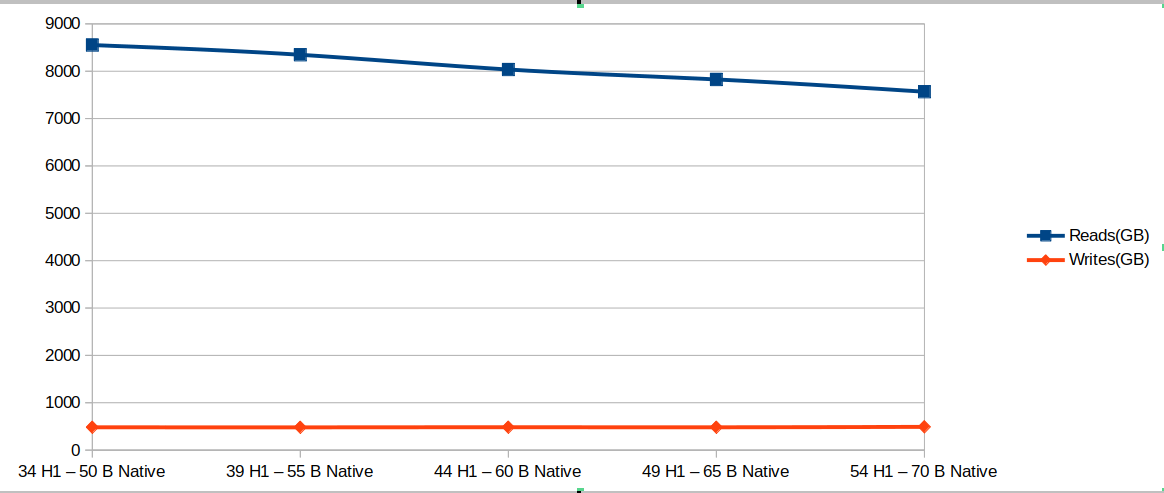
\includegraphics[width=\linewidth]{./fig/gcs_linr_h1_native.png}
    \caption{Number of Minor and Major GCs over heap size for H1 Linear Regression Native
    Spark investigation.}
    \label{fig:gcs_linr_h1_native}

    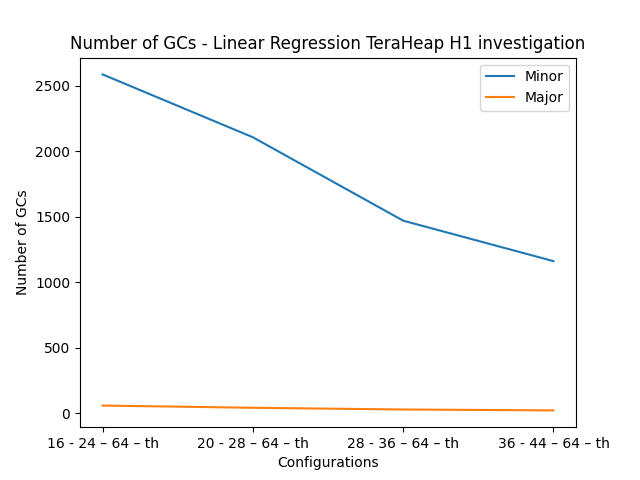
\includegraphics[width=\linewidth]{./fig/gcs_linr_h1_th.png}
    \caption{Number of Minor and Major GCs over heap size for H1 Linear Regression TeraHeap
    Spark investigation.}
    \label{fig:gcs_linr_h1_th}
\end{figure}

\begin{figure}[thbp]
    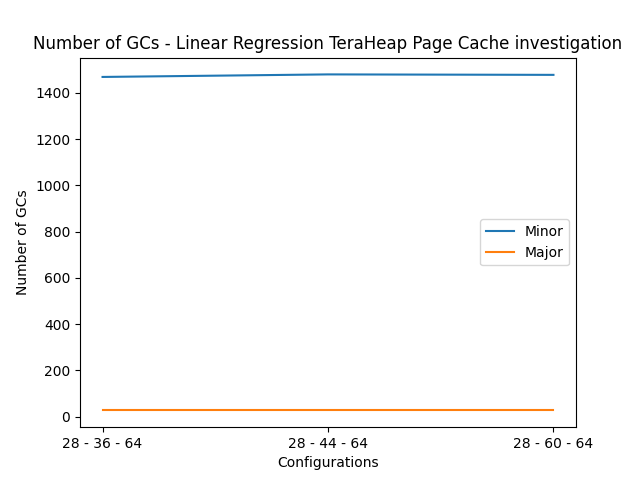
\includegraphics[width=\linewidth]{./fig/gcs_linr_pc_th.png}
    \caption{Number of Minor and Major GCs over heap size for Page Cache Linear Regression
    TeraHeap Spark investigation.}
    \label{fig:gcs_linr_pc_th}  

    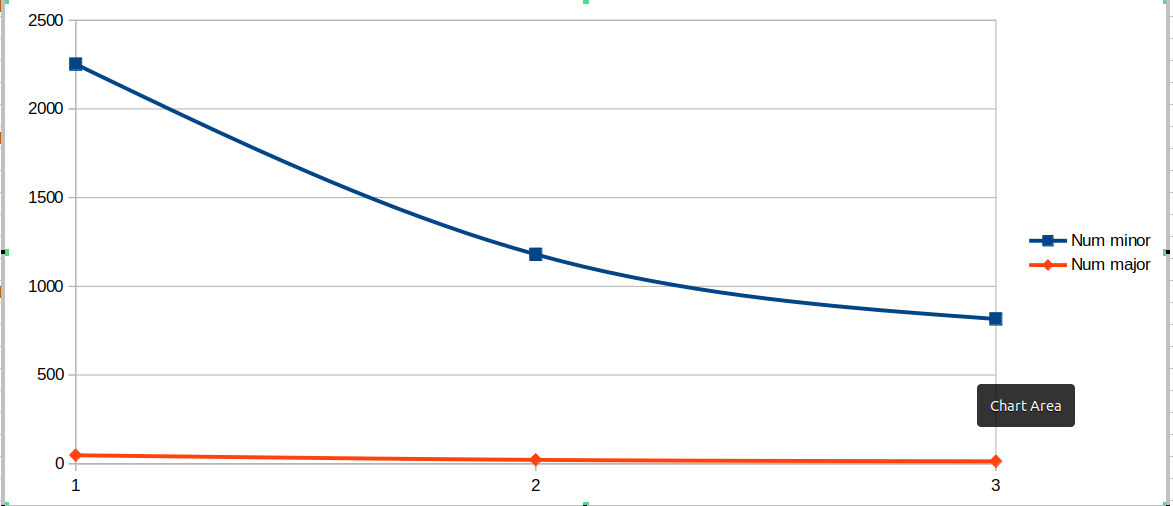
\includegraphics[width=\linewidth]{./fig/gcs_pr_h1_th.png}
    \caption{Number of Minor and Major GCs over heap size for H1 Page Rank TeraHeap Spark
    investigation.}
    \label{fig:gcs_pr_h1_th}
\end{figure}

\begin{figure}[thbp]
    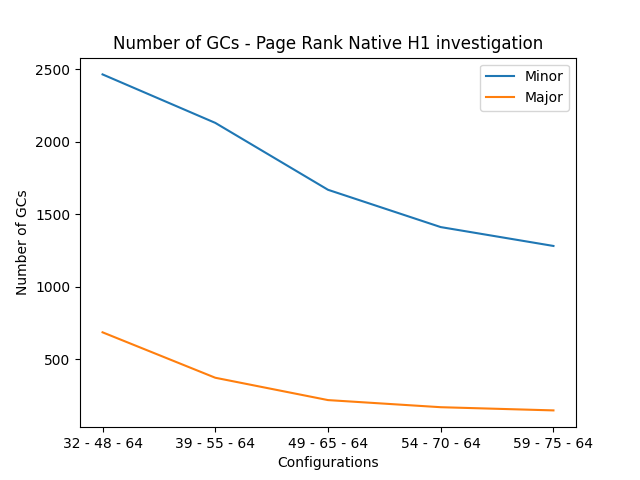
\includegraphics[width=\linewidth]{./fig/gcs_pr_h1_native.png}
    \caption{Number of Minor and Major GCs over heap size for H1 Page Rank Native Spark
    investigation.}
    \label{fig:gcs_pr_h1_native}

    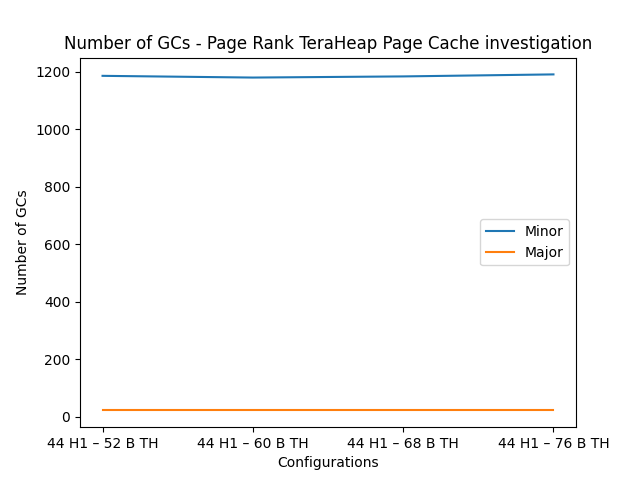
\includegraphics[width=\linewidth]{./fig/gcs_pr_pc_th.png}
    \caption{Number of Minor and Major GCs over Page Cache size for Page Cache Page Rank TeraHeap Spark
    investigation.}
    \label{fig:gcs_pr_pc_th}
\end{figure}

\begin{figure}[thbp]
    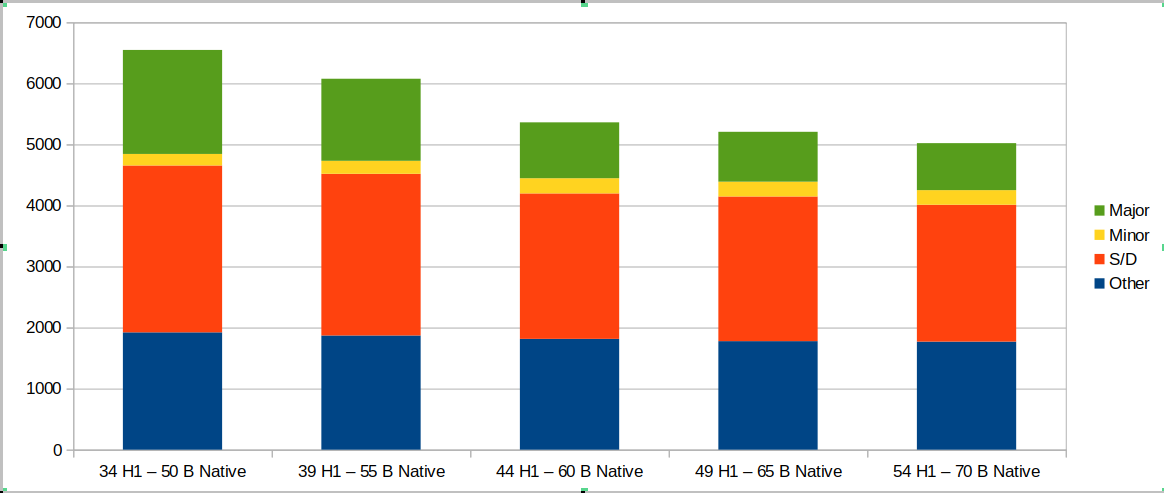
\includegraphics[width=\linewidth]{./fig/linr_h1_native.png}
    \caption{Execution time breakdown for H1 Linear Regression Native
    Spark investigation.}
    \label{fig:linr_h1_native}

    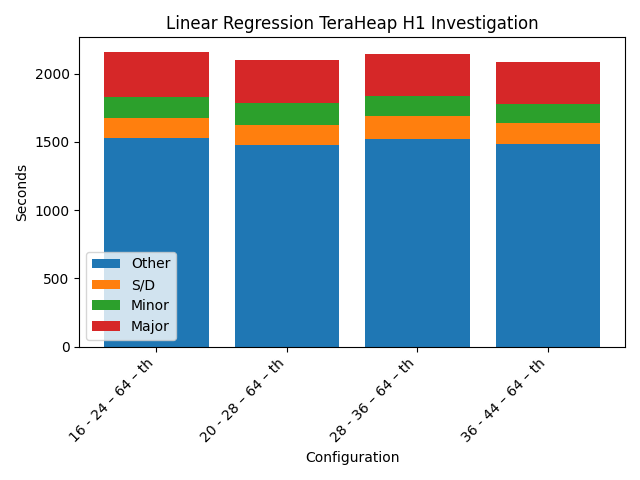
\includegraphics[width=\linewidth]{./fig/linr_h1_th.png}
    \caption{Execution time breakdown for H1 Linear Regression
    TeraHeap Spark investigation.}
    \label{fig:linr_h1_th}
\end{figure}

\begin{figure}[thbp]
    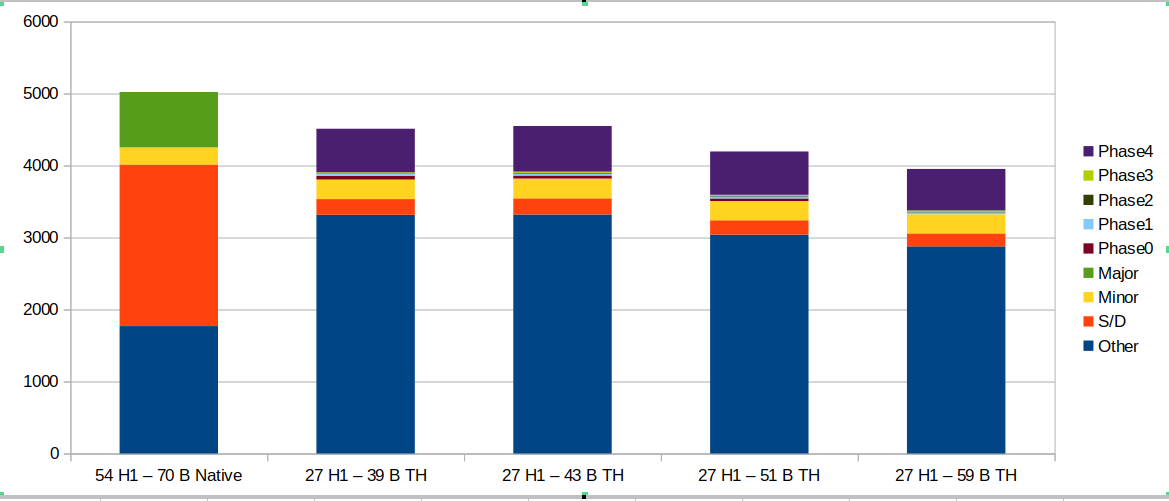
\includegraphics[width=\linewidth]{./fig/linr_pc_th.png}
    \caption{Execution time breakdown for Page Cache Linear Regression TeraHeap Spark investigation.}
    \label{fig:linr_pc_th}

    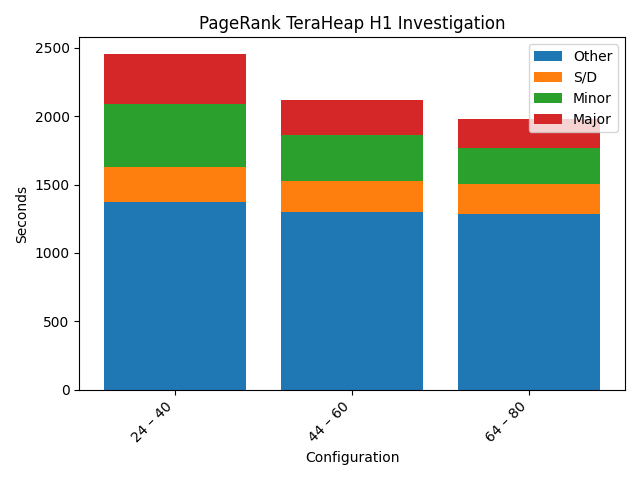
\includegraphics[width=\linewidth]{./fig/pr_h1_th.png}
    \caption{Execution time breakdown for H1 Page Rank TeraHeap Spark
    investigation.} 
    \label{fig:pr_h1_th}
\end{figure}

\begin{figure}[thbp]
    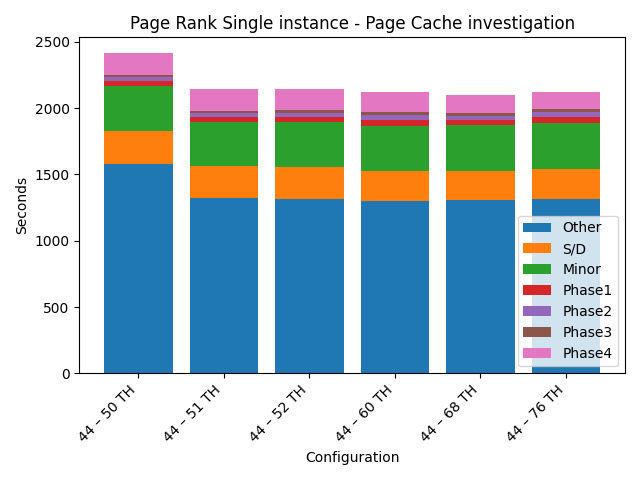
\includegraphics[width=\linewidth]{./fig/pr_pc_th.png}
    \caption{Execution time breakdown for PageCache Page Rank TeraHeap
    Spark investigation.}
    \label{fig:pr_pc_th}

    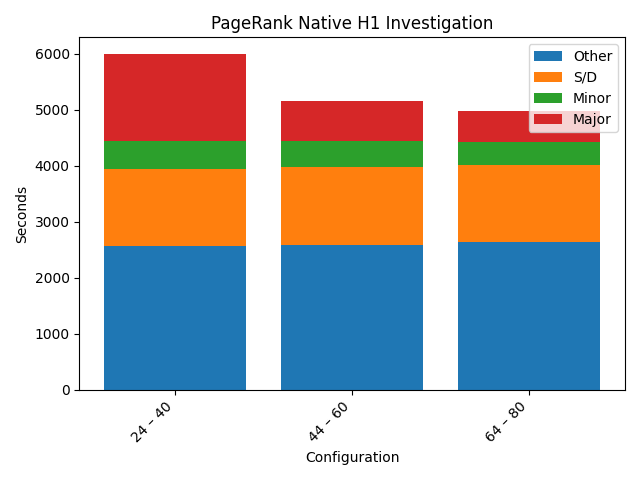
\includegraphics[width=\linewidth]{./fig/pr_h1_native.png}
    \caption{Execution time breakdown for H1 Page Rank Native
    Spark investigation.}
    \label{fig:pr_h1_native}
\end{figure}

\begin{figure}[thbp]
    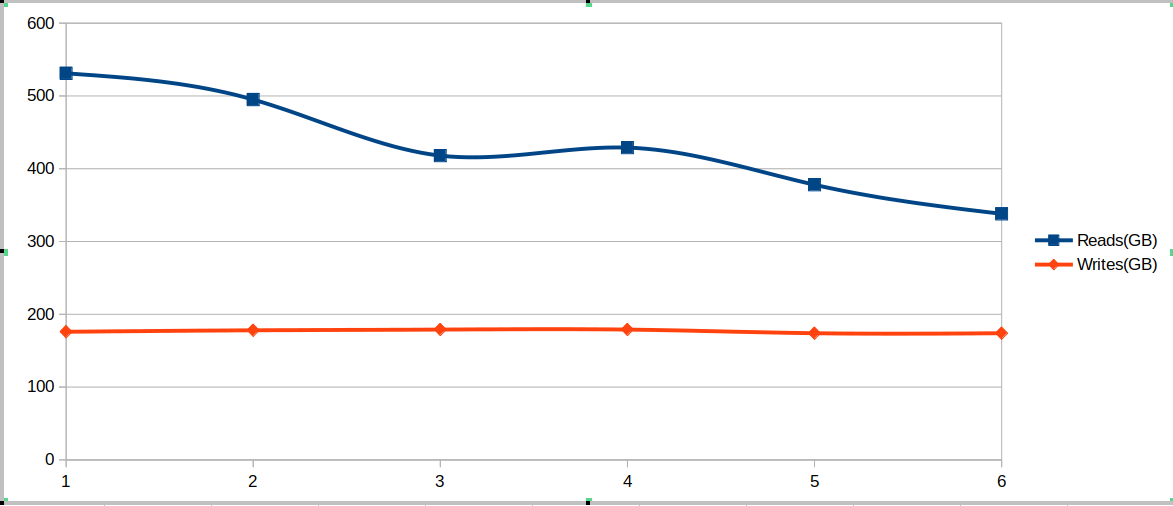
\includegraphics[width=\linewidth]{./fig/rw_pr_pc_th.png}
    \caption{Read-Write traffic over Page Cache size for PageCache Page Rank
    TeraHeap Spark investigation.}
    \label{fig:rw_pr_pc_th}

    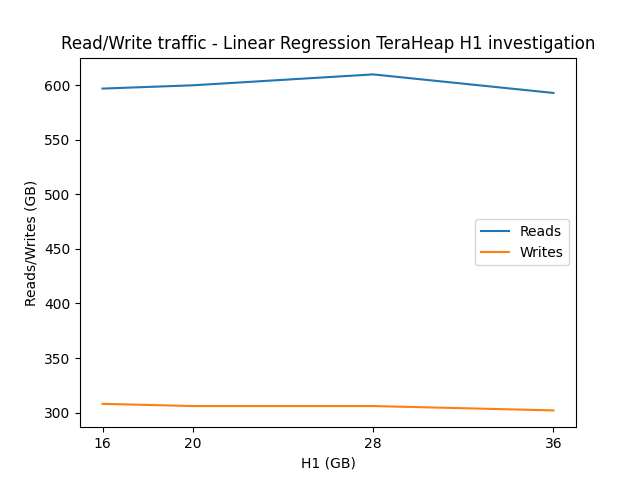
\includegraphics[width=\linewidth]{./fig/rw_linr_h1_th.png}
    \caption{Read-Write traffic over H1 size for H1 Linear Regression
    TeraHeap Spark investigation.}
    \label{fig:rw_linr_h1_th}
\end{figure}

\begin{figure}[thbp]
    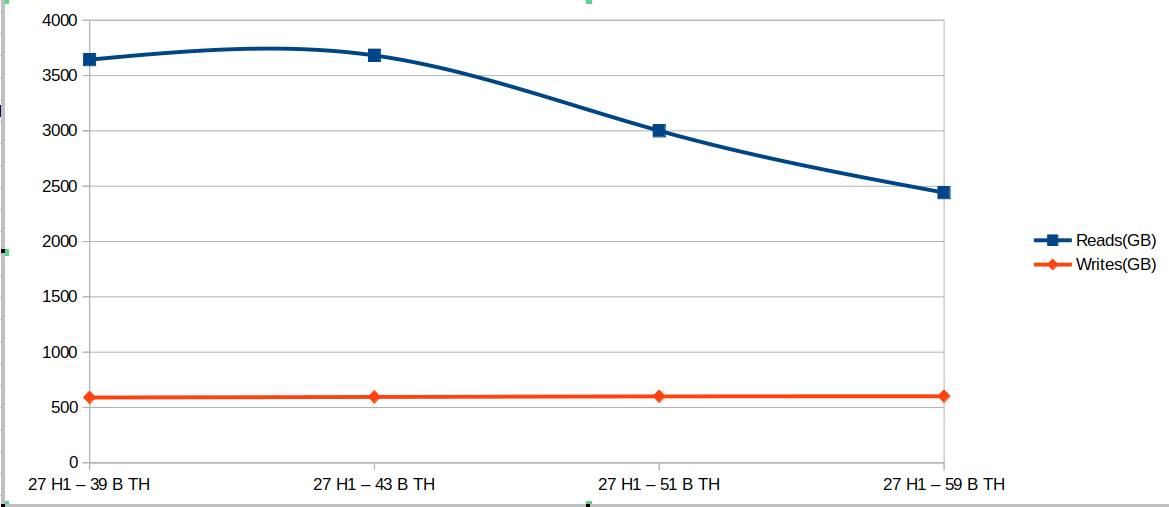
\includegraphics[width=\linewidth]{./fig/rw_linr_pc_th.png}
    \caption{Read-Write traffic over Page Cache size for PageCache Linear
    Regression TeraHeap Spark investigation. H1 is }
    \label{fig:rw_linr_pc_th}

    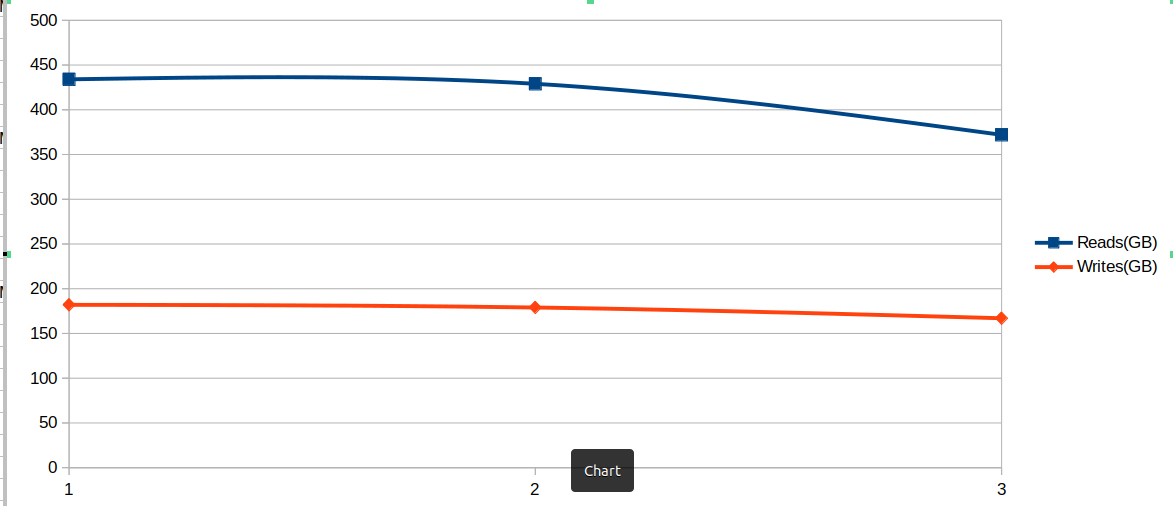
\includegraphics[width=\linewidth]{./fig/rw_pr_h1_th.png}
    \caption{Read-Write traffic over H1 size for H1 Page Rank TeraHeap
    Spark investigation.}
    \label{fig:rw_pr_h1_th}
\end{figure}
\fi

\iffalse
\subsection{Spark investigation}
Spark's memory management is critical for the performance of big data
analytics applications. In Spark, memory is divided into two
regions: execution memory, and storage memory. Execution memory
is used for storing data during shuffle and join operations and for
caching frequently accessed data. Storage memory is used for storing long lived
cached data. Additionally, Spark uses a combination
of in-memory and disk-based storage to provide efficient data access.
Spark provides various storage levels, including MEMORY-ONLY,
MEMORY-AND-DISK, and DISK-ONLY, to allow users to balance between
memory usage and data availability. We choose MEMORY-AND-DISK for Native Spark 
to cache 50\% of the RDDs in memory and 50\%s off-heap, in the storage device,
to balance memory and storage usage. Spark needs significant amounts
of memory even with the use of an off-heap compute cache. Since our spark applications run within a
memory-limited cgroup in order to assure fair performance in-between
isolated workloads, that means that we have to investigate how the different
Spark workloads are performing with different amounts of H1 (Java Heap) for Native-TeraHeap Spark ann I/O cache for Native-TeraHeap Spark.
Increasing/decreasing H1 automaticaly does the opposite to the I/O
cache, because of the cgroup memory limit. 
We condut this investigation to choose the appropriate configuration to run the co-located experiments.
The appropriate configuration is the one with the optimal performance.
We find this configuration by hand by exploring how H1 and Page Cache affect 2 workloads.
We do this by keeping one of the metrics stable to a certain value and we then adjust the other.
We break the execution time to Major GC, Minor GC and Other time which includes time going to IO from applications threads.

Figure \ref{fig:pr_h1_native} shows performance of single-instance Native Spark
running PageRank with adjustable size for H1 while available DRAM for the rest of the services is kept
steady at 16 GB. This graph shows that decreasing the size of H1
indicates a significant increase to Major GC. Both the second and the third configuration
increase performance by 20\% compared to the first. However the second consumes
30\% more DRAM when the third consumes 50\% more DRAM. We therefore choose the second configuration
as it provides same performance with the third and less DRAM consumption.
Figure \ref{fig:gcs_pr_h1_native} justifies the Major GC changes by showing the obvious
decrease of the number of major gcs.

Figure \ref{fig:pr_h1_th} shows performance of single-instance TeraHeap Spark
running PageRank with adjustable size for H1 while avalaible DRAM for Page Cache is kept
steady at 16 GB. This graph shows that decreasing the size of H1
indicates a significant increase to Minor GC and a slight increase to
Major GC. 
The second and third configuration consume 30\% and 50\% more DRAM than the first,
and they provide 15\% and 20\% speedup accordingly. We choose the second configuration 
due to increased performance and only slightly higher DRAM consumption than the third.
Figure \ref{fig:gcs_pr_h1_th} justifies the difference in Major GC time by showing the obvious
decrease of the number of minor gcs. 

Figure \ref{fig:pr_pc_th} shows performance of
single-instance TeraHeap Spark running PageRank with adjustable size
for Page Cache while H1 is kept steady at 44 GB. This graph shows that
decreasing the size of PageCache indicates no changes to other time.
All configurations have the same performance. Therefore we choose the second
which is directly comparable to the one we chose for TeraHeap, despite not being the ideal in terms
of total need in DRAM. We do this to help ourselves analyze the performance of the co-located workloads using this configuration.
Figure \ref{fig:rw_pr_pc_th} justifies these claims by showing read-traffic to be steady.

Figure \ref{fig:linr_h1_native} shows performance of single-instance
Native Spark running LinearRegression with adjustable size for H1
while PageCache is kept steady at 8 GB. This graph shows that
decreasing the size of H1 indicates a significant increase to Major GC
and a slight increase to S/D. Other time remains the same.
The last 2 bars speedup execution by 30\% while consuming more than 50\% of DRAM.
Therefore we choose the last which consumes a slightly lower DRAM budget.
Figure \ref{fig:gcs_linr_h1_native} justifies the behaviour of Major GC by showing the number of minor-major gcs to decrease
while H1 increases (gc time). 

Figure \ref{fig:linr_h1_th} shows performance of
single-instance TeraHeap Spark running LinearRegression with
adjustable size for H1 while PageCache is kept steady at 8 GB. This
graph shows that decreasing the size of H1 indicates no increase to
GC. 
All configurations provide the nearly the same performance with slight changes.
Therefore we choose the second because it is the most optimal in combination with
low DRAM consumption. 
Figure \ref{fig:gcs_linr_h1_th} and \ref{fig:rw_linr_h1_th}
justify these numbers by showing the number of major gcs to stay the
same while H1 increases (gc time) and the read-write traffic to remain
steady (other). 
Figure \ref{fig:linr_pc_th} shows performance of
single-instance TeraHeap Spark running LinearRegression with
adjustable size for PageCache while H1 is kept steady at 28 GB. This
graph shows that decreasing the size of PageCache indicates no changes
to Other time. So changes to PageCache do not affect this workload.
All configurations pose no differences to execution time so we choose the 
third one despite consuming more DRAM. We do this because it is directly comparable
in terms of DRAM budget with the one we have chosen for Native Spark for this workload.
Figure \ref{fig:gcs_linr_pc_th} and \ref{fig:rw_linr_pc_th} justify
these numbers by showing the number of minor-major gcs as well as
read-write traffic to remain the same.

\subsubsection{Giraph Investigation}
\begin{figure}[thbp]
    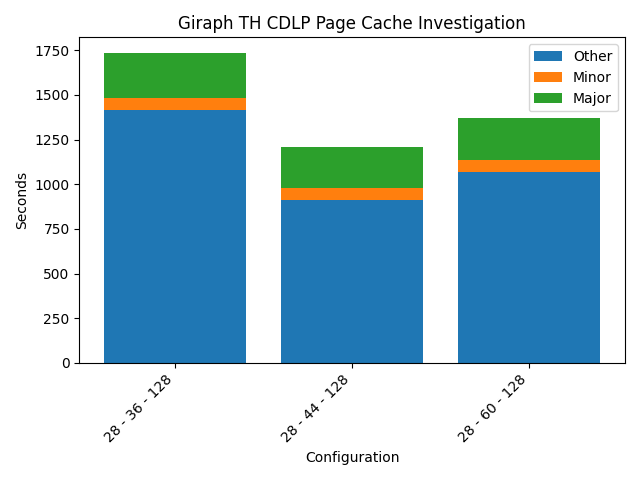
\includegraphics[width=\linewidth]{./fig/g_pr_pc_th.png}
    \caption{Execution time breakdown for PageCache PR TeraHeap
    Giraph investigation.}
    \label{fig:g_pr_pc_th}

    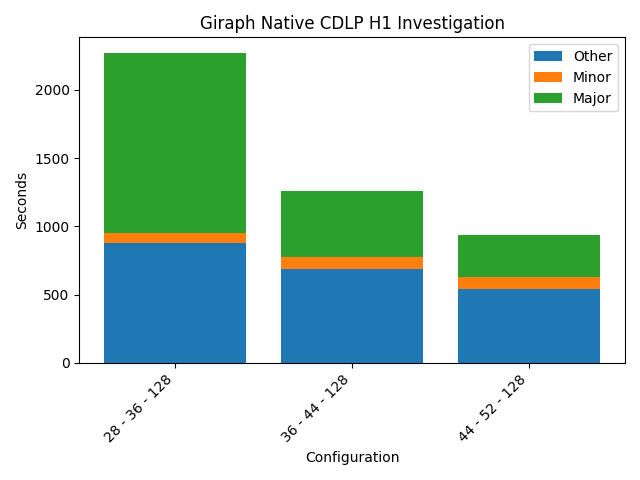
\includegraphics[width=\linewidth]{./fig/g_pr_h1_native.png}
    \caption{Execution time breakdown for H1 PR Native
    Giraph investigation.}
    \label{fig:g_pr_h1_native}
\end{figure}

\begin{figure}[thbp]
    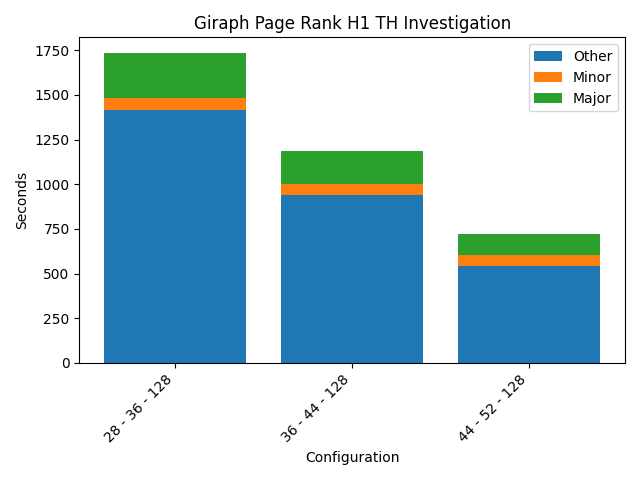
\includegraphics[width=\linewidth]{./fig/g_pr_h1_th.png}
    \caption{Execution time breakdown for PageCache PR TeraHeap
    Giraph investigation.}
    \label{fig:g_pr_pc_th}

    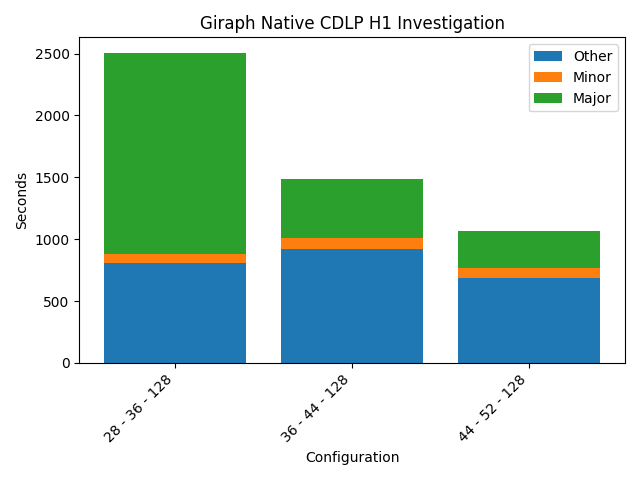
\includegraphics[width=\linewidth]{./fig/g_cdlp_h1_native.png}
    \caption{Execution time breakdown for H1 CDLP Native
    Giraph investigation.}
    \label{fig:g_pr_h1_native}
\end{figure}
\fi

\iffalse
\subsection{Metrics} 
When measuring performance, it's
important to choose metrics that provide a comprehensive view of the
system's behavior. In the case of measuring the performance of Spark and Giraph
colocated instances, there are several key metrics that one should consider.
These include heap capacity, which is the amount of memory allocated
GC time is also an
important metric, as it measures the amount of time spent by the JVM
garbage collector in freeing up memory. Serialization/deserialization
time, measured using Java async-profiler \cite{Profiler}, is important for
understanding how much time is spent in this operation, which can be a
bottleneck for some workloads. Other time, which is simply the
difference between total time and GC and serialization/deserialization
time, can provide insight into other factors that may be affecting
performance, but mainly includes the time spent in I/O and also the
time spent by mutator threads to run the application code. Device
traffic, measured using iostat, is important for understanding how
much data is being read from and written to storage devices. CPU idle
and IO wait, measured using mpstat, can help identify how much of the
CPU and I/O resources are being utilized. Finally, average throughput,
measured using Spark Bench, is a good indicator of the overall
performance of the system. Other metrics, such as the total amount of
data processed and the number of minor and major garbage collections,
as measured using jstat, can also provide valuable insights into
system behavior. By considering a range of metrics, one can get a more
accurate and comprehensive view of the performance of Spark instances.
\fi
\iffalse
\subsection{Benefits of colocating instances} 
Concurrent execution of workloads provides several benefits.
Firstly, it enables optimal resource utilization by effectively
leveraging the available hardware resources, including CPUs, memory,
and storage. Rather than leaving server resources idle between
workloads, concurrent execution ensures their efficient utilization,
leading to improved throughput and enhanced server efficiency.
Additionally, the consolidation of multiple workloads onto a single
server reduces hardware footprint, simplifies management, and
minimizes operational costs associated with managing multiple servers.

Another advantage is the potential for increased throughput. By
executing multiple workloads concurrently, tasks progress
simultaneously, resulting in faster completion and higher overall
throughput. This approach is particularly valuable when workloads
exhibit varying levels of computational intensity or have different
resource requirements. Concurrent execution allows for efficient
resource allocation, enabling each workload to access the necessary
resources and perform optimally.

Concurrent execution also facilitates workload prioritization,
allowing organizations to allocate resources based on workload
importance or urgency. By running multiple workloads concurrently,
critical or high-priority tasks can be assigned the required resources
and processed in a timely manner. This flexibility in resource
allocation and workload prioritization ensures efficient utilization
of available resources and improves overall performance.

Furthermore, the concurrent execution of workloads supports
experimentation and testing. By running workloads concurrently on the
same server, comparisons, performance benchmarking, and optimization
can be performed in a controlled environment. This concurrent
execution environment enables organizations to evaluate and fine-tune
applications effectively.

Moreover, concurrent execution of workloads allows users to run
workloads along with other users simultaneously. While this is a
method that wouldn't be considered correct in order to evaluate
something because of the interference of other applications running
concurrently, it is something common for the cloud and datacenters
where companies-users share the cloud-server.

Scalability is another advantage of concurrent execution. As data
volumes and processing demands increase, running multiple workloads
concurrently allows for horizontal scalability. Additional 
worker nodes can be added to accommodate larger workloads or handle
additional workloads without the need for significant infrastructure
changes. This scalability ensures that the system can handle growing
demands while maintaining high performance.

In conclusion, the concurrent execution of multiple workloads on
a single server offers significant advantages for performance
optimization. It enables optimal resource utilization, workload
consolidation, improved throughput, workload prioritization,
experimentation, and scalability. By carefully managing resources,
workload scheduling, and monitoring, organizations can achieve higher
performance, reduce infrastructure costs, and simplify management.
\fi

\subsection{Cost estimation}
Renting servers is a common practice for organizations requiring
computational resources, and the question arises as to whether
reducing the monetary cost is possible by achieving higher throughput
and faster workload completion. The relationship between cost
reduction and achieving higher throughput on rented servers is indeed
significant. By optimizing server performance, efficiently utilizing
resources, implementing workload scheduling, and improving
productivity, organizations can realize cost savings. Achieving higher
throughput and faster workload completion can lead to a reduced rental
duration, minimizing the time and associated costs of server usage.
Efficient resource utilization and workload scheduling contribute to
cost reduction by minimizing the number of servers required and
maximizing their utilization. Rental pricing models that take into
account resource utilization or data processed can further reduce
costs for organizations achieving higher throughput. Additionally,
improved productivity resulting from higher throughput and faster
workload completion enhances overall efficiency, allowing
organizations to accomplish more work within the same rental period
and reducing rental expenses. Therefore, pursuing higher throughput
and faster workload completion offers tangible benefits in terms of
monetary cost reduction for organizations renting servers. 

In order to estimate the cost of our evaluation in real-world public clusters we
chose a variety of providers like Amazon \cite{EC2}, Google \cite{GCP} and Microsoft \cite{Azure}. This
way we covered the most known providers and platforms someone would
choose to run their workloads on. We chose 2 machines from each
platform identical to the specifications of our 64, 128 and 256 GB DRAM
machines. These are the cheapest machines of that particular category
offered by the platform. We then used the platform's pricing
calculator to estimate the cost of renting that machine for the time
needed for each configuration to finish execution of all instances. We noticed that the price for
renting the storage device is really amenable to the cost for renting the machine.
